\chapter{Задача слежения за гармоническим сигналом (регулятор общего вида)}

Рассмотрим замкнутую систему с регулятором общего вида:
\[
H(s) = \frac{\sum_{k=0}^m b_k s^k}{\sum_{k=0}^n a_k s^k} = \frac{N_{reg}(s)}{D_{reg}(s)}
\]
Для задающего воздействия $g(t) = \sin(0.25 t)$ синтезируем физически 
реализуемый регулятор, способный обеспечить предельное значение ошибки 
$e_{\text{уст}} = 0$.

Найдем образ Лапласа для $g(t)$:
\[
G(s) = \frac{0.25}{s^2 + 0.25^2} = \frac{N_g(s)}{D_g(s)}
\]

Выберем $D_{reg}$ так, чтобы $D_{reg}\cdot D$ включали в себя корни $D_g$:
\[
D_{reg}(s) = D(s) \cdot D_g(s) = s^2 + 0.25^2
\]

Выберем $N_{reg}$ так, чтобы корни $D_{reg}\cdot D + N_{reg}\cdot N$ 
были отрицательными. Так как система должна быть физически реализуемой
$N_{reg}$ будет иметь вид:
\[
N_{reg}(s) = a_2 s^2 + a_1 s + a_0
\]

Передаточная функция замкнутой системы относительно ошибки:
\[
W_{g\to e}(s) = \frac{1}{1+W(s)W_{reg}(s)} 
= \frac{1}{1 + \frac{1}{2s^2 + 3s + 1} \frac{a_2 s^2 + a_1 s + a_0}{s^2 + 0.25^2}}
=
\]
\[
= \frac{(2s^2 + 3s + 1)(16s^2 + 1)}{(2s^2 + 3s + 1)(16s^2 + 1) + 16(a_2 s^2 + a_1 s + a_0)}
=
\]
\[
= \frac{(2s^2 + 3s + 1)(16s^2 + 1)}{32s^4 + 48s^3 + (18 + 16a_0)s^2 + (3 + 16a_1)s + 1 + 16a_2}
\]

Применим критерий Гурвица:
\[
    \Delta_1 = 48 > 0
\]
\[
    \Delta_2 = 
    \begin{vmatrix}
        48 & 3 + 16a_1 \\
        32 & 18 + 16a_0
    \end{vmatrix}
    = 48(18 + 16a_0) - 32(3 + 16a_1) =
    768 + 768a_0 - 512a_1 >0
\]
\[
    \Delta_3 = 
    \begin{vmatrix}
        48 & 3 + 16a_1 & 0 \\
        32 & 18 + 16a_0 & 1 + 16a_2 \\
        0 & 48 & 3 + 16a_1
    \end{vmatrix}
    = 2304a_{0}+10752a_{1}-36864a_{2}+12288a_{0}a_{1}
    -
    \]\[
    -8192{a_{1}}^2> 0
\]
\[
    \Delta_4 = 
    \begin{vmatrix}
        48 & 3 + 16a_1 & 0 & 0 \\
        32 & 18 + 16a_0 & 1 + 16a_2 & 0 \\
        0 & 48 & 3 + 16a_1 & 0 \\
        0 & 32 & 18 + 16a_0 & 1 + 16a_2
    \end{vmatrix}
    = 256(16a_2 + 1)*(9a_0 + 42a_1 - 144a_2 
    +
    \]\[
    + 48a_0a_1 - 32a_1^2)> 0
\]

Возьмем такие значения $a_0$, $a_1$ и $a_2$, которые удовлетворяют условиям:
\[
a_0 = 0,\, a_1 = 1,\, a_2 = 0
\]
\[
H(s) = \frac{s}{2s^2 + 3s + 1}
\]

Аналитически рассчитаем установившуюся ошибку:
\[
e_{\text{уст}} = \lim_{s \to 0} s W_{g\to e}(s) 
= \lim_{s \to 0} s \frac{0.25}{s^2 + 0.25^2} \frac{(2s^2 + 3s + 1)(16s^2 + 1)}{32s^4 + 48s^3 + 18s^2 + 19s + 1} = 0
\]

Составим схему моделирования в Simulink и выполним моделирование:
\begin{figure}[H]
    \centering
    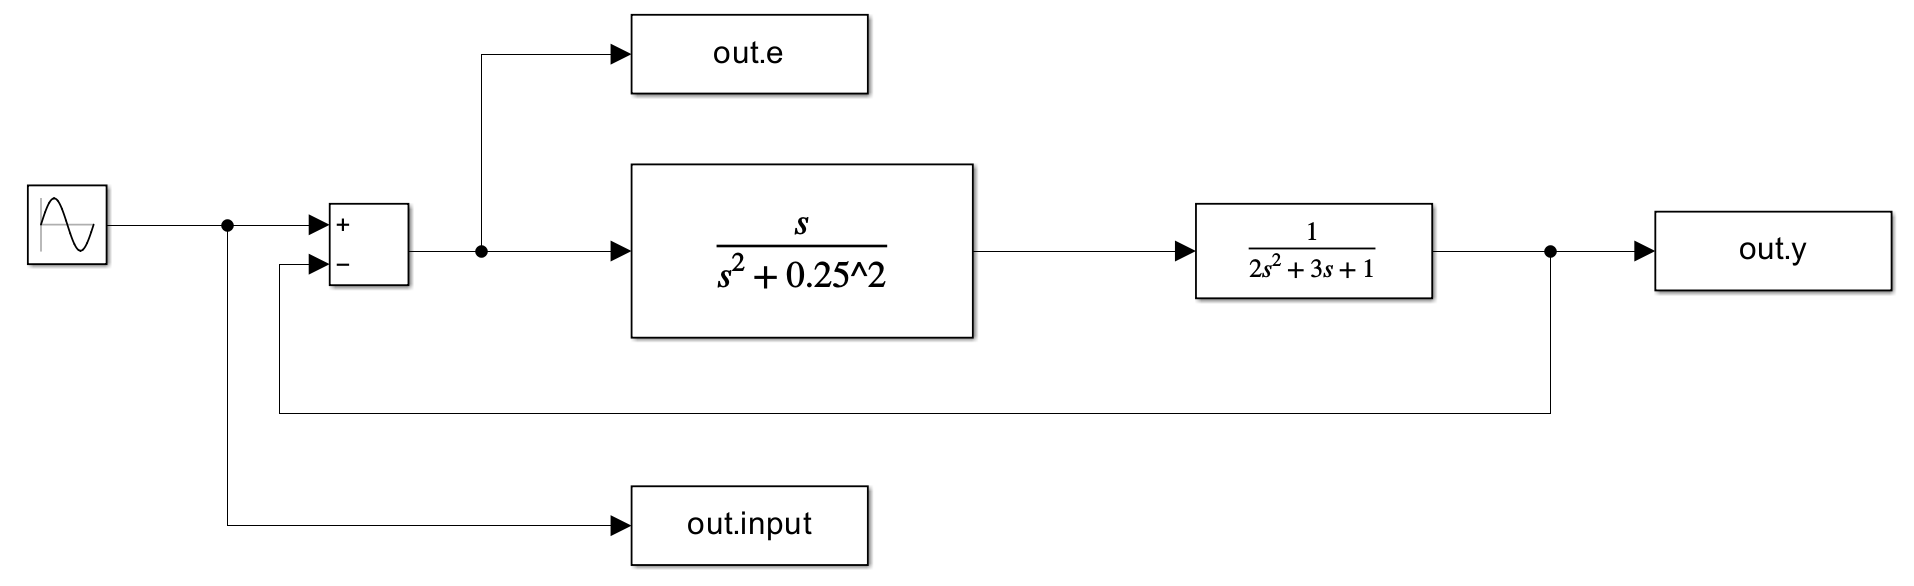
\includegraphics[width=1\textwidth, trim={0cm 0cm 0cm 0cm}]{../images/sim5.png}
    \caption{Схема моделирования}
\end{figure}
\begin{figure}[H]
    \centering
    \begin{minipage}{0.45\textwidth}
        \centering
        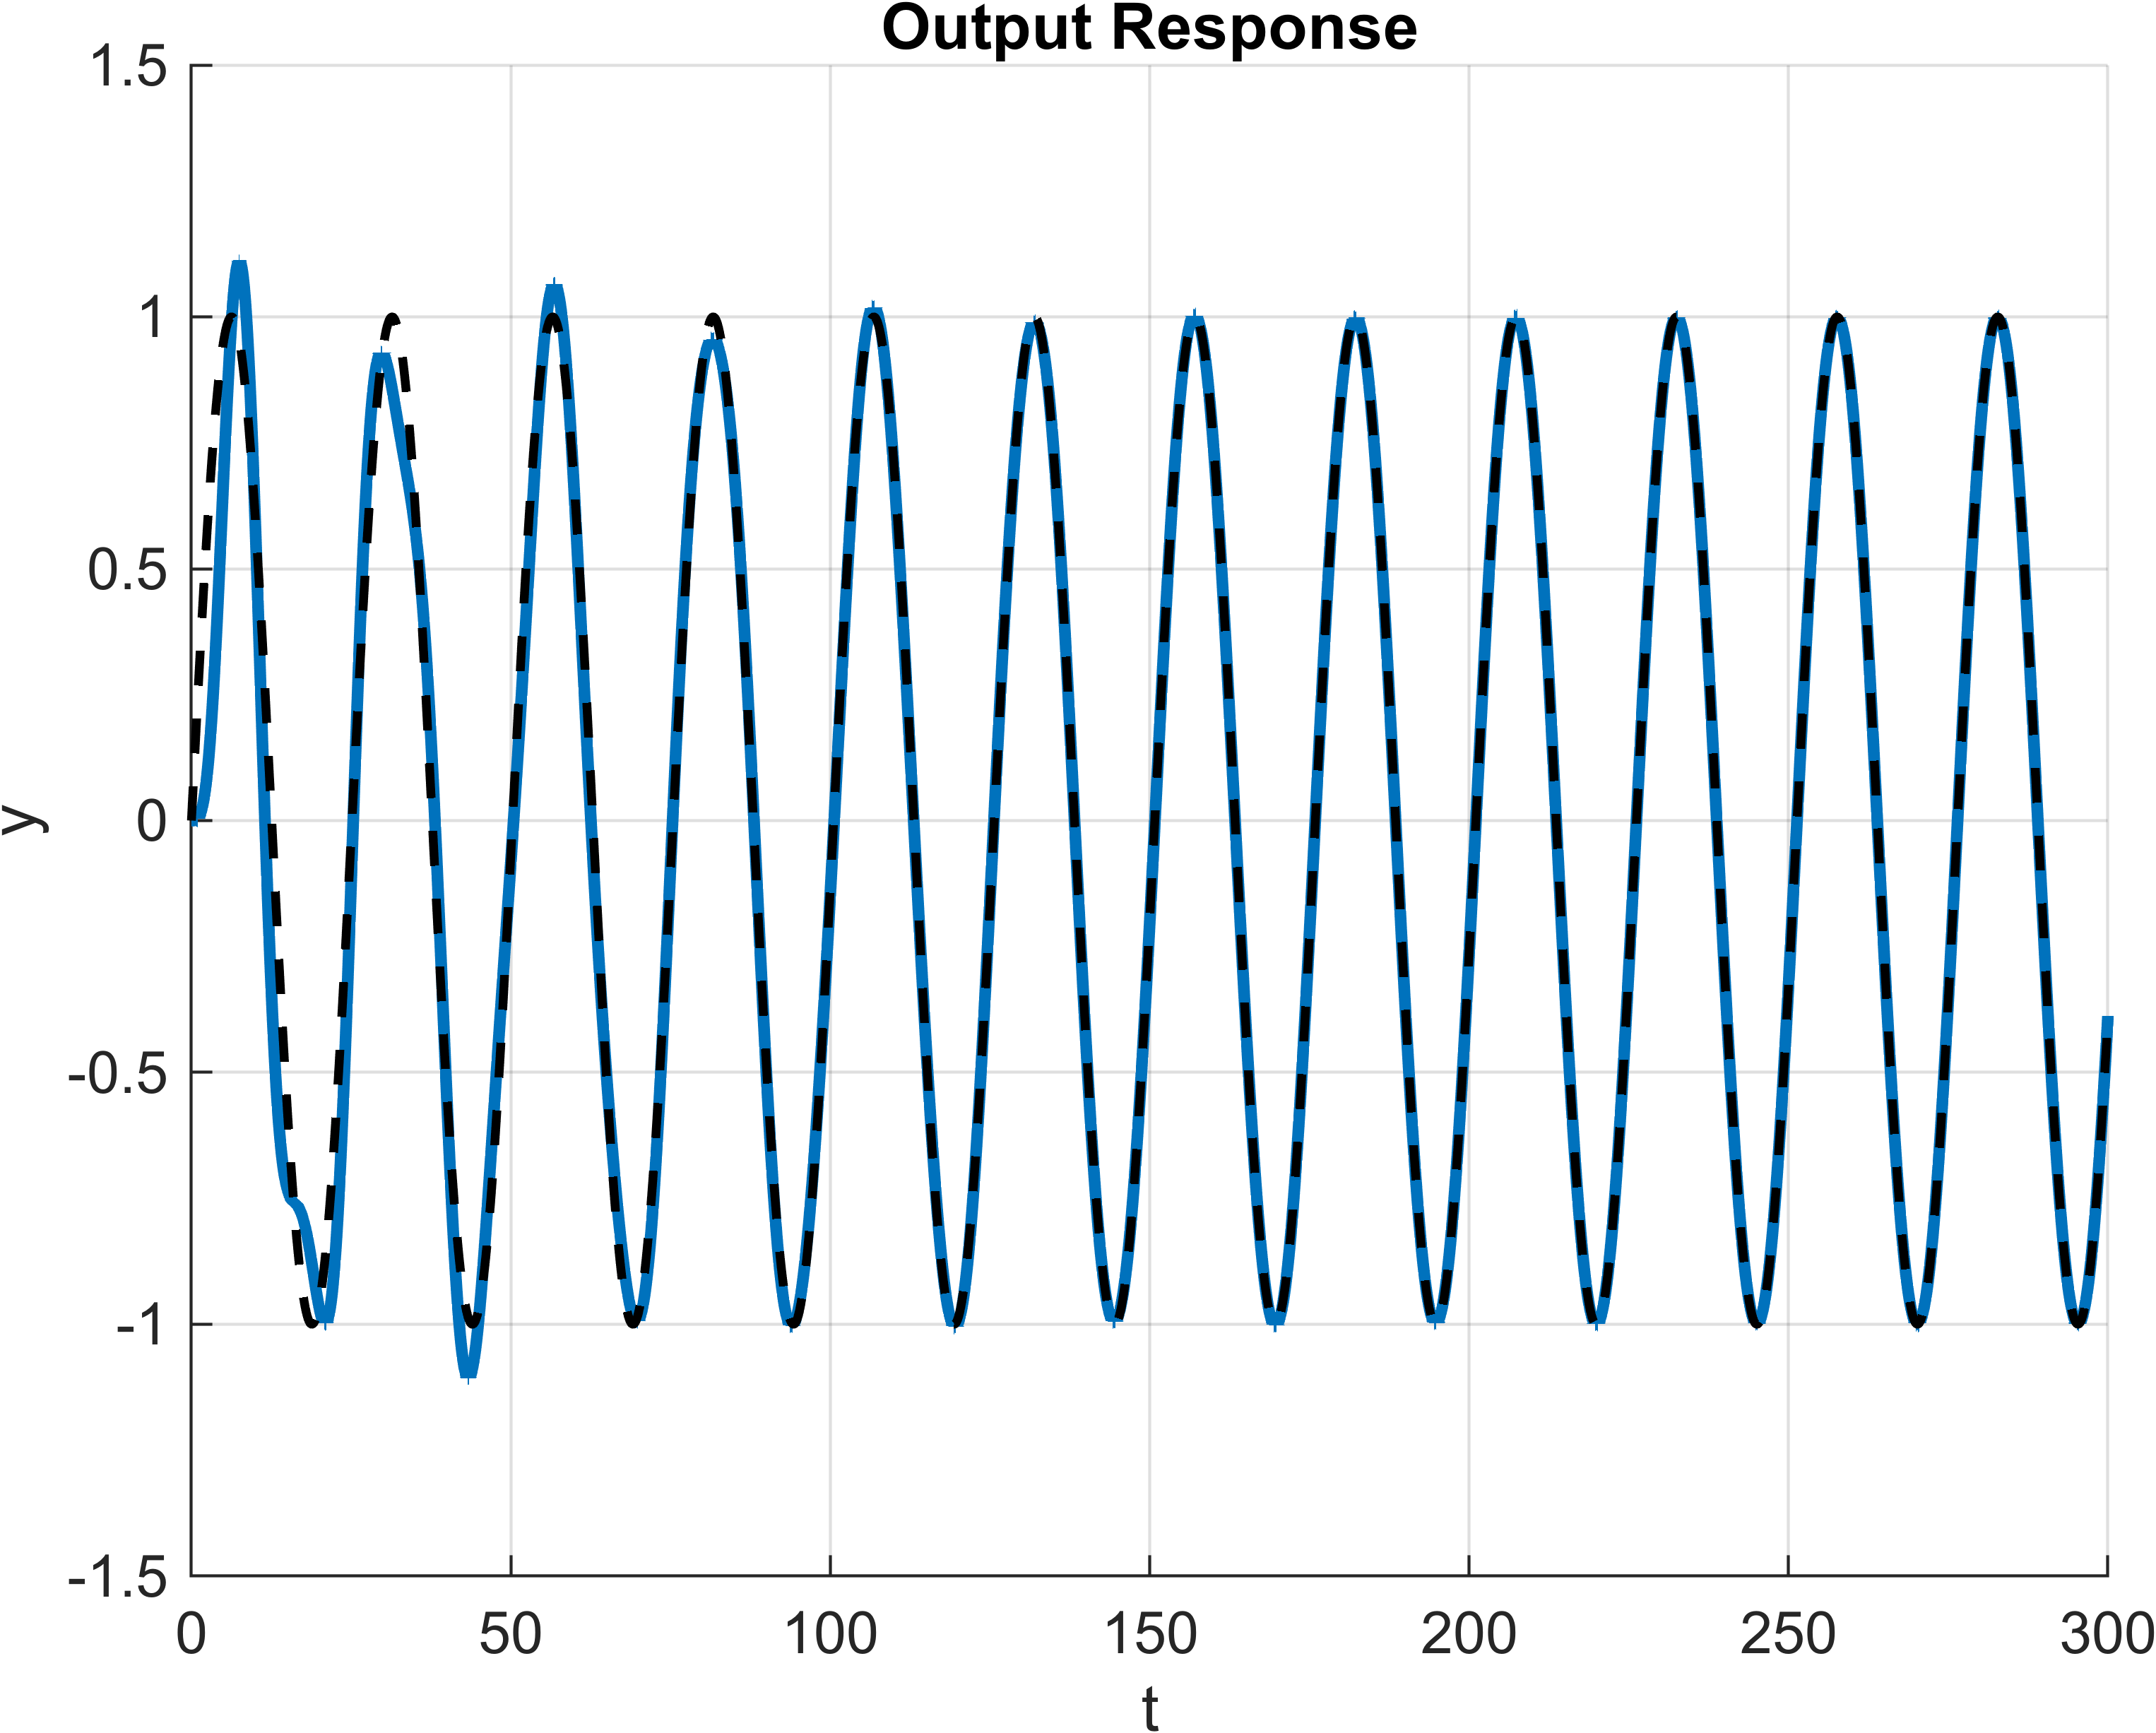
\includegraphics[width=1\textwidth, trim={1cm 0cm 1cm 0cm}]{../images/6_1.png}
    \end{minipage}
    \hfill
    \begin{minipage}{0.45\textwidth}
        \centering
        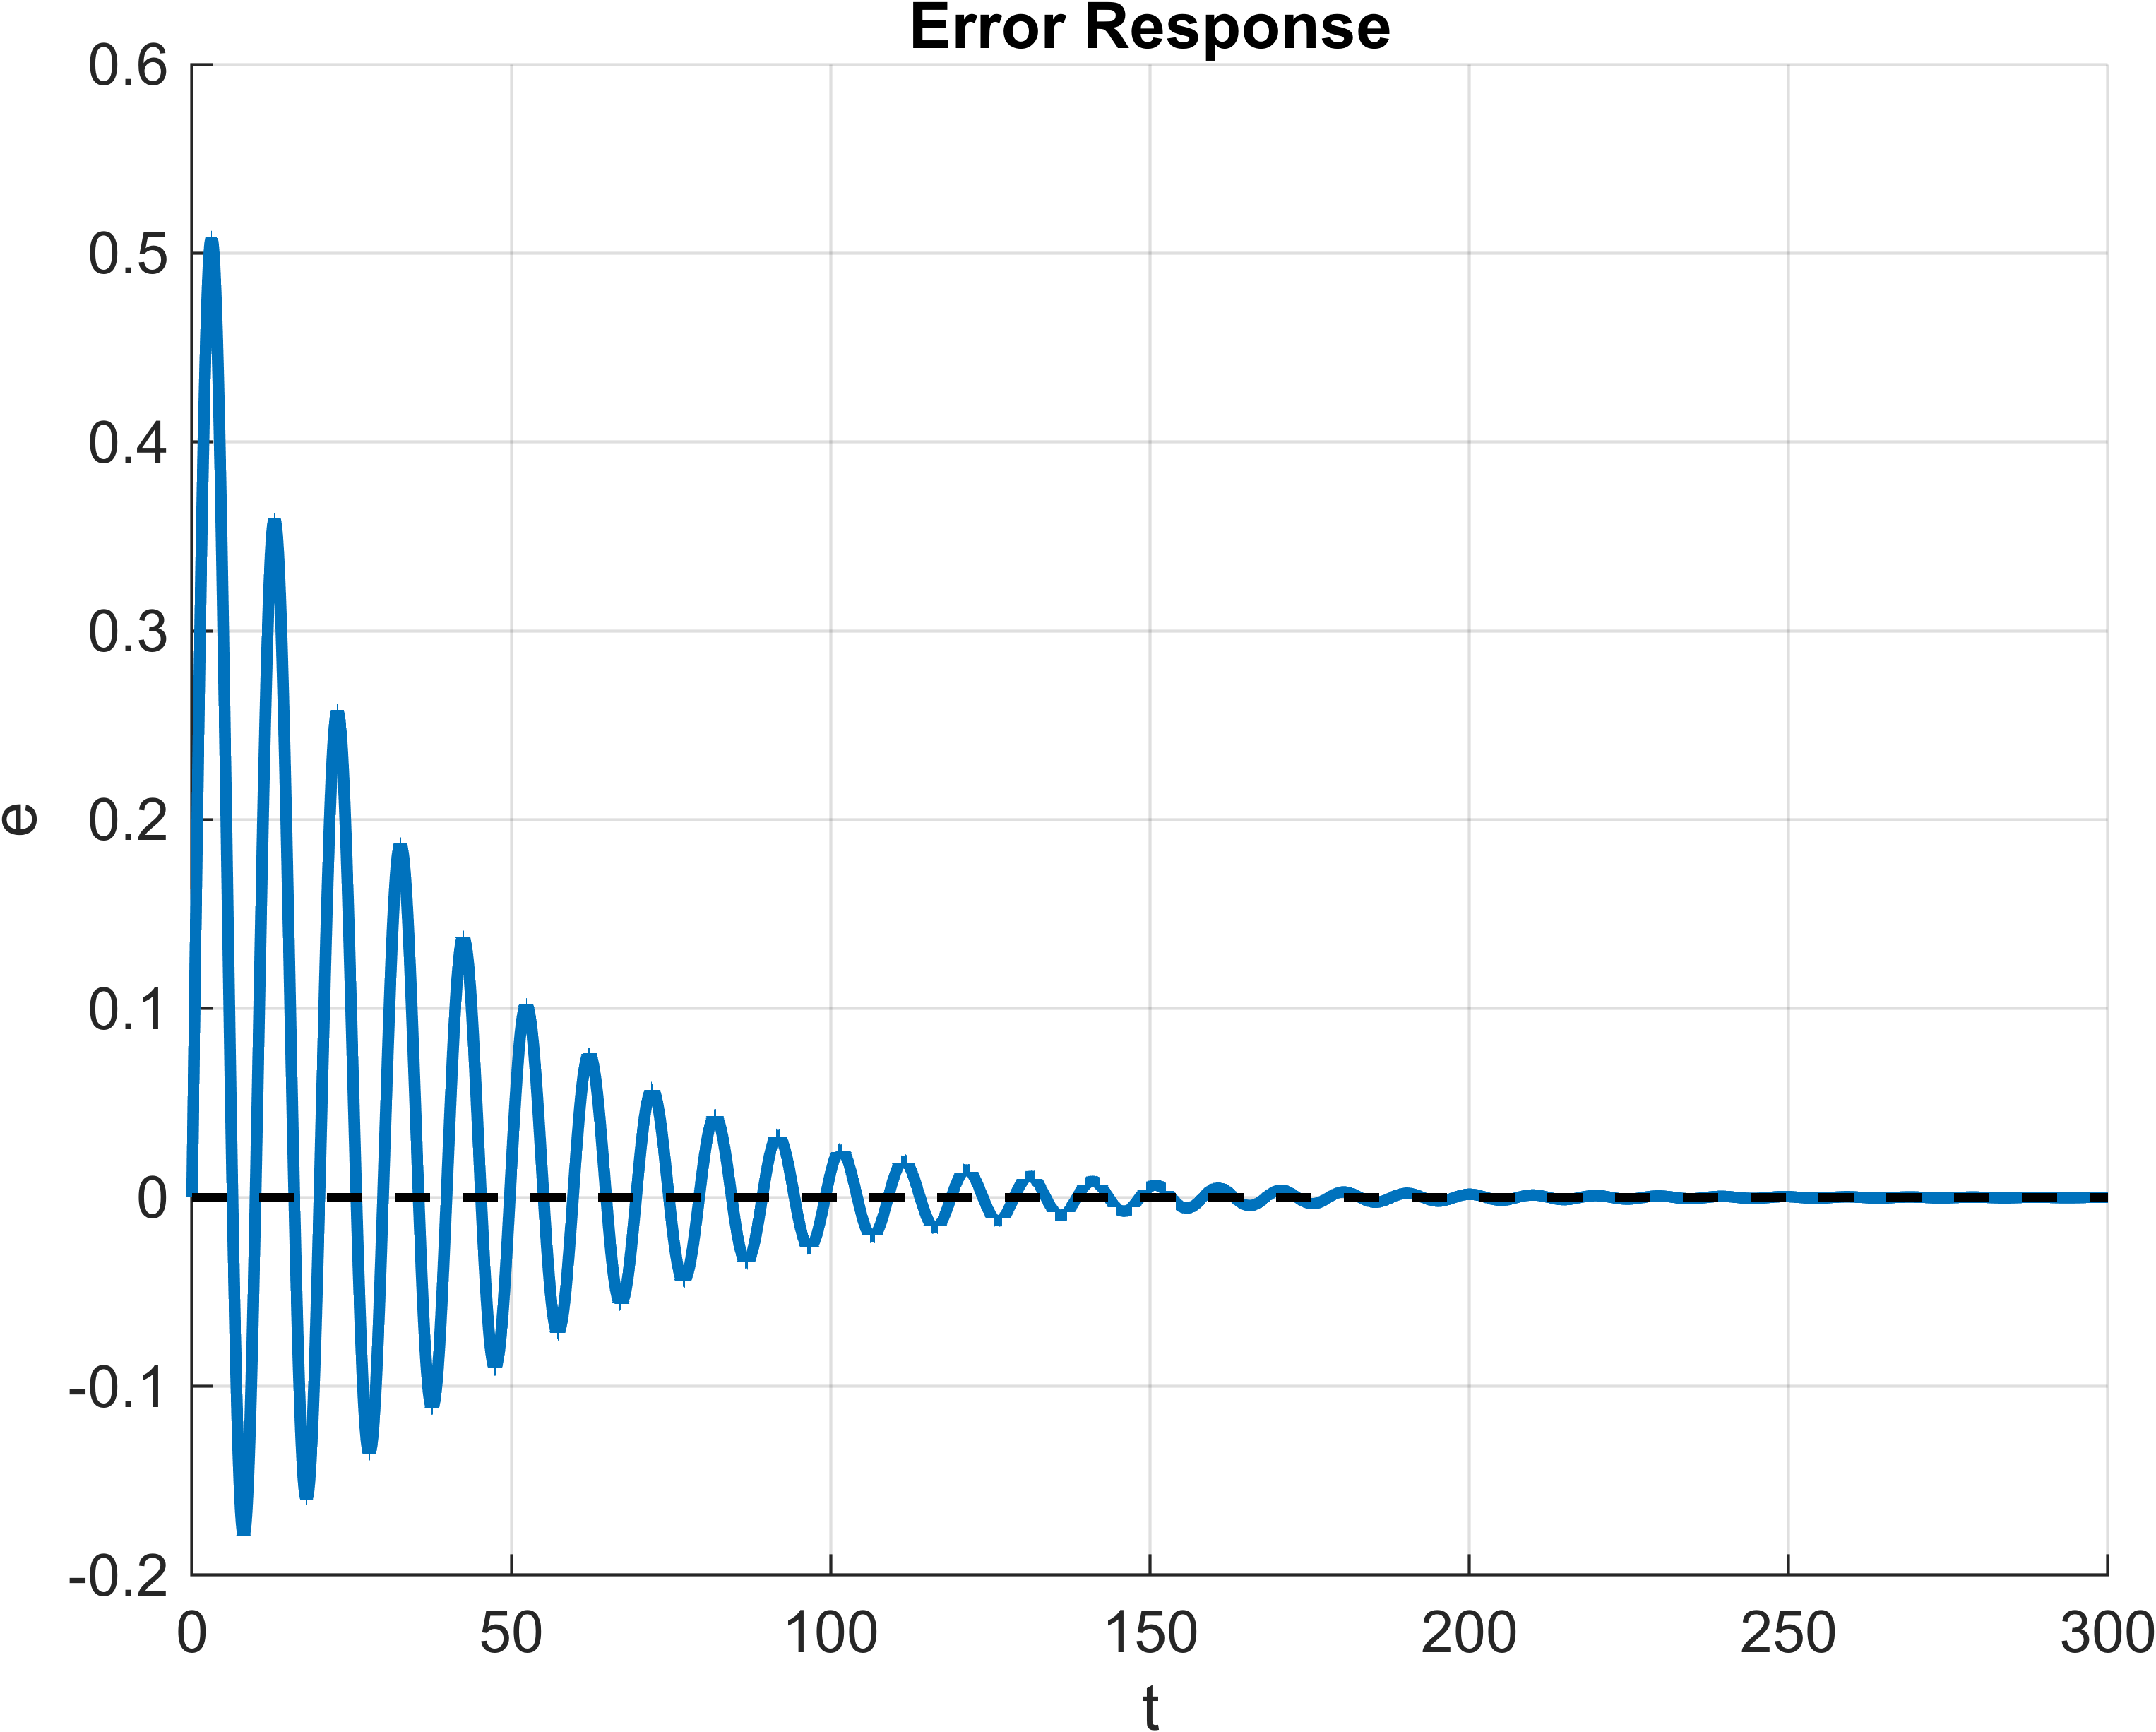
\includegraphics[width=1\textwidth, trim={1cm 0cm 1cm 0cm}]{../images/6_2.png}
    \end{minipage}
    \caption{Графики $y(t)$ и $e(t)$ при $g(t) = \sin(0.25t)$}
\end{figure}

Как видим из аналитических расчетов и графиков, синтезированный регулятор 
обеспечивает нулевую установившуюся ошибку. Однако, коэффициенты были выбраны
не самые оптимальные, так как система имеет перерегулирование и довольно 
большое время переходного процесса.
\endinput